\documentclass{article} 
\usepackage{hyperref}
\usepackage{tikz} 
\usepackage{amsmath}
\usepackage{amssymb} 
\usepackage[ a4paper]{geometry}
\usepackage{fancyhdr}
\pagestyle{fancy}
\lhead{Skalarprodukte}
\rhead{April 2025 - Juli 2025}
\begin{document}
  
\newcommand{\norm}[1]{\big| {#1} \big|}  
\newcommand{\vect}[1]{\overrightarrow{#1}} 
 
\section{Skalarprodukte}
Das Skalarprodukt von zwei Vektoren beschreibt die Summe aller Produkte der jeweiligen Koordinatenpaare der Vektoren. Es gilt
\begin{align*}
 \vect{a} \cdot \vect{b} &=
 a_1 \cdot b_1 + a_2 \cdot b_2 && \text{in der zweiten Dimension} \\
 \vect{a} \cdot \vect{b} &=
 a_1 \cdot b_1 + a_2 \cdot b_2 + a_3 \cdot b_3 && \text{in der dritten Dimension}
\end{align*}
In der Regel sind Skalarprodukte ausschließlich in der dritten Dimension relevant. 
 
\subsection{Orthogonalität}
\begin{description} 
 \item[Vektoren] Zwei Vektoren sind zueinander orthogonal, heißt senkrecht, wenn sie ein Skalarprodut von $0$ haben. \newline
 Wie später im Kapital \hyperref[Winkel]{Winkel} weiter erklärt wird ist das Skalarprodut vom $\cos$ des Winkels zwischen den beiden Vektoren abhängig. Demnach haben Vektoren, welche ungefähr in die gleiche Richtung zeigen, ein positives Skalarprodukt, weil $\alpha < 90^\circ \Rightarrow \cos{(\alpha)} > 0$, Vektoren, welche in die ungefähr entgegengesetze Richtung zeigen, ein negatives Skalarprodukt, weil $\alpha > 90^\circ \Rightarrow \cos{(\alpha)} < 0$ und Vektoren, welche in einem $90^\circ$ Winkel zueinander stehen, ein Skalarprodukt von $0$, weil $\alpha = 90^\circ \Rightarrow \cos{(\alpha)} = 0$. 
\end{description}
\begin{center}
 \begin{tabular}{p{4cm} p{4cm} p{4cm}}
  \centering 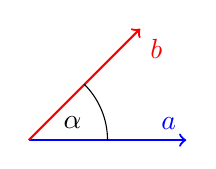
\begin{tikzpicture}
   \draw[->,thick,blue] (0,0) -- ++(2, 0) node [above left] {$\vect{a}$};
   \draw[->,thick,red] (0,0) -- ++({2*sin(45)},{2*cos(45)}) node [below right] {$\vect{b}$};
   \draw (1, 0) arc[start angle=0,end angle=45,radius=1];
   \draw ({0.6*sin(67.5)},{0.6*cos(67.5)}) node {$\alpha$};
  \end{tikzpicture}
  &
  \centering 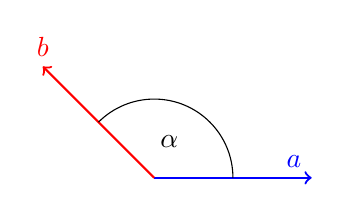
\begin{tikzpicture}
   \draw[->,thick,blue] (0,0) -- ++(2, 0) node [above left] {$\vect{a}$};
   \draw[->,thick,red] (0,0) -- ++({2*sin(-45)},{2*cos(-45)}) node [above] {$\vect{b}$};
   \draw (1, 0) arc[start angle=0,end angle=135,radius=1];
   \draw ({0.5*sin(22.5)},{0.5*cos(22.5)}) node {$\alpha$}; 
  \end{tikzpicture} 
  &
  \makebox[4cm][c]{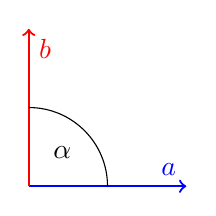
\begin{tikzpicture}
   \draw[->,thick,blue] (0,0) -- ++(2, 0) node [above left] {$\vect{a}$};
   \draw[->,thick,red] (0,0) -- ++(0, 2) node [below right] {$\vect{b}$};
   \draw (1, 0) arc[start angle=0,end angle=90,radius=1];
   \draw ({0.6*sin(45)},{0.6*cos(45)}) node {$\alpha$};
  \end{tikzpicture}}
  \\
  \centering $\alpha < 90^\circ$ &
  \centering $\alpha > 90^\circ$ &
  \makebox[4cm][c]{ $\alpha = 90^\circ$} \\
  \centering $\vect{a} \cdot \vect{b} > 0$ &
  \centering $\vect{a} \cdot \vect{b} < 0$ &
  \centering $\vect{a} \cdot \vect{b} = 0$
 \end{tabular} 
\end{center} 
  
\noindent \begin{minipage}{3.5cm}
 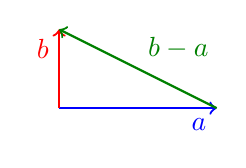
\begin{tikzpicture}
  \centering 
  \draw[->,thick,blue] (0,0) -- (2, 0) node [below left] {$\vect{a}$};
  \draw[->,thick,red] (0,0) -- (0, 1) node [below left] {$\vect{b}$};
  \draw[->,thick,green!50!black] (2,0) -- (0, 1) node [midway, above right] {$\vect{b}-\vect{a}$};
 \end{tikzpicture}  
\end{minipage}
\hfill
\begin{minipage}{\dimexpr\linewidth-3.5cm}
 Desweiteren kommt dies daher, dass die Enden von zwei orthogonalen Vektoren $\vect{a}$ und $\vect{b}$ miteinander Verbunden werden können, um mit dem $\vect{ab} = \vect{b} - \vect{a}$ ein rechtes Dreieck zu bilden. Somit gilt dem Satz von Pythagoras nach  
 \[  
  \norm{\vect{a}}^2 + \norm{\vect{b}}^2 = \norm{\vect{b} - \vect{a}}^2
 \]
 
\end{minipage}
Weiterhin folgt darauf
\begin{align*}
 a_1^2+a_2^2+b_1^2+b_2^2 &= (b_1-a_1)^2 + (b_2-a_2)^2 && \vert\,\text{2. bin Formel} \\
   &= b_1^2-2b_1a_1+a_1^2 + b_2^2-2b_2a_2+a_2^2 && \vert\,-(a_1^2+a_2^2+b_1^2+b_2^2) \\
 0 &= -2b_1a_1 + -2b_2a_2 && \vert\, :(-2) \\
 0 &= a_1b_1+a_2b_2 
\end{align*}
 
\begin{description}
 \item[Geraden] Zwei Geraden verlaufen zueinander, wenn ihre jeweiligen Richtungsvektoren zueinander orthogonal sind. Sie müssen sich nicht zwangsweise schneiden.
 \item[Gerade und Ebene] Eine Gerade verläuft zu einer Ebene orthogonal, wenn der Richtungsvektor der Gerade zu beiden Richtungsvektoren der Ebene orthogonal ist. Genau dies macht, per definition, der Normalvektor einer Ebene. Somit ist eine Gerade auch orthogonal zu einer Ebene, wenn der Richtungsvektor der Gerade zum Normalvektor der Ebene kollinear ist, welches, falls der Normalvektor bereits gegeben ist, schneller zu berechnen sein kann. 
\end{description} 
\end{document}  
 
